\chapter{Tutorial}

\section{Adsorption isotherm of N$_2$ in a metal-organic framework (MOF), Henry coefficients, enthalpy of adsorption}


\begin{figure}[H]
  \centering
  \subfloat[]{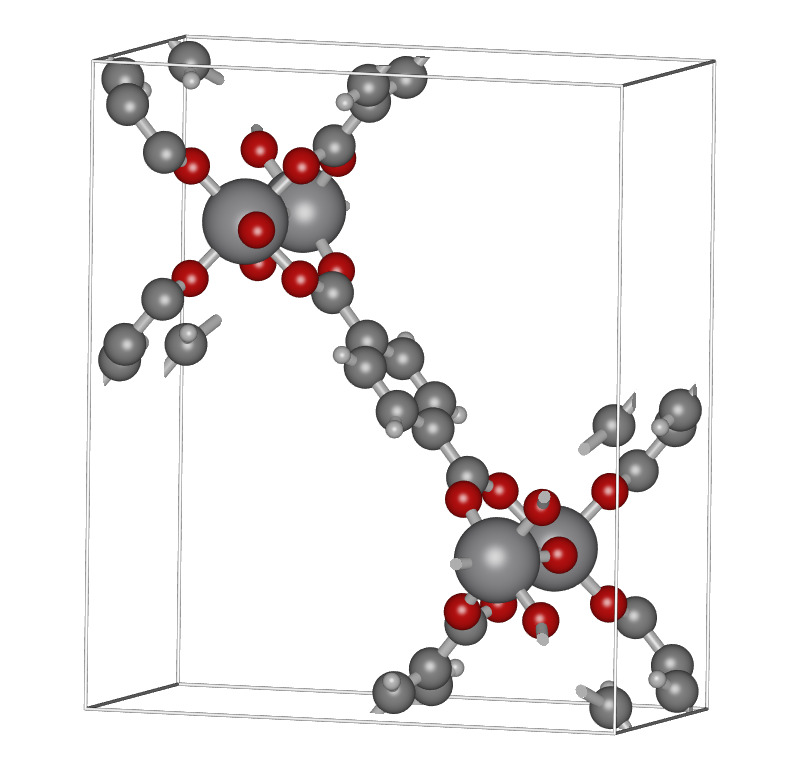
\includegraphics[width=7.5cm]{./Tutorial/MIL-47.jpg}}
  \subfloat[]{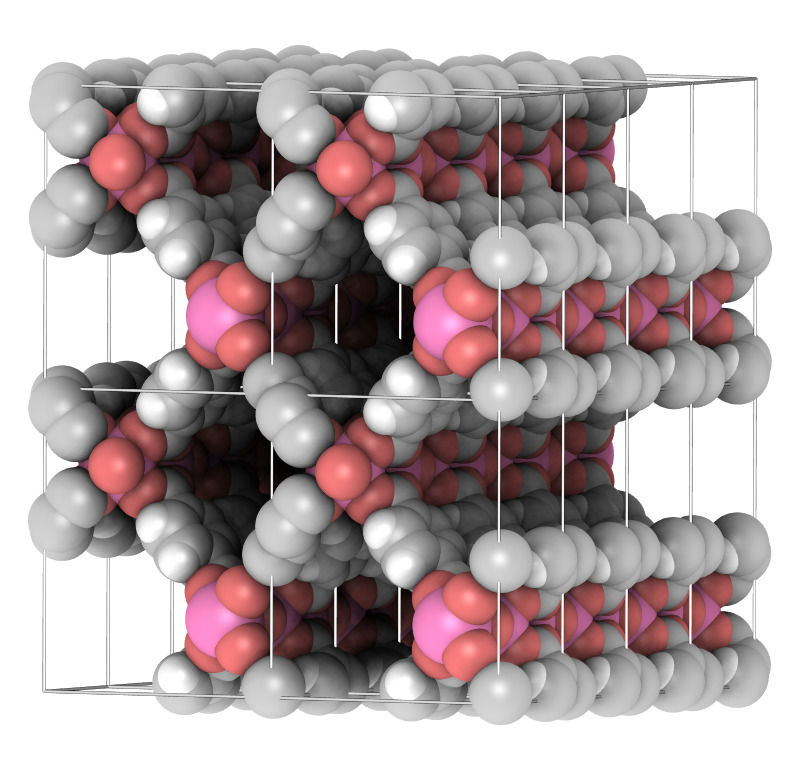
\includegraphics[width=7.5cm]{./Tutorial/MIL-47-2x2x4.jpg}}
  \caption{(left) The MIL-47 unit cell, $6.8179\times 16.1430 \times 13.9390$ \AA, $\alpha=\beta=\gamma=90^\circ$, (right) the $4\times2\times2$ supercell.}
  \label{Tutorial-MIL-47.jpg}
\end{figure}

We are going to look at adsorption properties of methane in MIL-47 \cite{Barthelet2002}. The MIL-47 structure is shown in Fig. \ref{Tutorial-MIL-47.jpg}.
The first step is to select the size of the system. We are going to choose a VDW cutoff of 12 \AA. This implies that all \emph{perpendicular} lengths
of the unit cell should be larger than twice the cutoff, i.e.\ 24 \AA. So, as a \emph{minimum}, we should use at least a $4\times2\times2$ unit cells.
This requirement follows from the "minimum-image convention" where the interactions are computed with only the closest periodic image.

\begin{table}[t]
\begin{tabularx}{\linewidth}{X|X|X|X|X}
type &   V$^{0+}$    &  V$^{2+}$    & V$^{4+}$     & DFT \\
\hline
V    &   2.67677     &  1.45833     &  1.83592     &  1.68 \\
O1   &  -0.986909    & -0.527963    & -0.661157    & -0.6  \\
O2   &  -0.712381    & -0.439958    & -0.516643    & -0.52 \\
O3   &  -0.693279    & -0.427135    & -0.501819    & -0.52 \\
C1   &   0.00680379  & -0.0146643   & -0.0110838   & -0.15 \\
H1   &   0.0434488   &  0.0574796   &  0.055858    &  0.12 \\
C2   &   0.0116383   & -0.0118276   & -0.00782077  & -0.15 \\
H2   &   0.0444475   &  0.0586772   &  0.0570134   &  0.12 \\
C3   &  -0.150672    & -0.0720208   & -0.083311    &  0.0 \\
C4   &   0.605064    &  0.384265    &  0.420426    &  0.56 \\
\end{tabularx}
\caption{Obtaining charges for MIL-47: charge equilibration vs. DFT-derived charges.}
\label{Tutorial-charges}
\end{table}

The positions of the atoms are usually known from experiments, or alternatively can be obtained from QM optimizations.
Using the atomic information of the framework only, we can compute the frameworks-mass as 14787.6 g mol$^{-1}$, 
and we can already compute a few interesting properties. 
The first is a measurement of how void the structure is.

\begin{center}
\shadowbox{%
\begin{minipage}[c]{15cm}
Exercise 1: go to the sub-directory '\verb+1-Helium-void-fraction+'. Compute the helium void-fraction
(look for `\verb+Rosenbluth factor new: 0.608 [-]+' in the output file).
\end{minipage}}
\end{center}

About 61\% of the structure is empty!

\begin{center}
\shadowbox{%
\begin{minipage}[c]{15cm}
Exercise 2: go to the sub-directory '\verb+1-Helium-void-fraction+'. Add a line '\verb+HeliumVoidFraction 0.61+' below '\verb+Framework 0+',
use zero cycles, and check the structural properties (i.e.\ accesible pore volume and loading conversion factors) of the system.'
\end{minipage}}
\end{center}

We see that the available pore volume is 0.60977519 cm$^3$ g$^{-1}$. This density is important to know, because, using the liquid density,
it gives a first approximation of the "maximum" number of molecules in the pore.

Two other very useful properties are the accessible surface and pore-size distribution.
\begin{center}
\shadowbox{%
\begin{minipage}[c]{15cm}
Exercise 3: go to the sub-directory '\verb+3-Surface-area+'. Run and compute the surface area.
\end{minipage}}
\end{center}

The nitrogen surface area of MIL-47 is about 1650 m$^2$ g$^{-1}$. This is much larger than most zeolites, but smaller than most large pore MOFs
which can go up to an incredible 5000-7000 m$^2$ g$^{-1}$.

\begin{center}
\shadowbox{%
\begin{minipage}[c]{15cm}
Exercise 4: go to the sub-directory '\verb+4-Pore-size-distribution+'. Run and compute the pore-size-distribution.
Plot the output-file in '\verb+PoreSizeDistributionHistogram+' in gnuplot using column 1 vs.\ 3
(\verb+plot 'PoreSizeDistributionHistogram' us 1:3 with lines+) to see what the typical pore sizes are.
\end{minipage}}
\end{center}

In general, the individual framework atoms are charged, but the overall framework should be charge neutral (or compensated by cations when the
framework itself has a net-charge).
For the charges there is ambiguity, since charge is not an ab-initio observable. That means that different methods to obtain charges
give different answers. For adsorption however, we are not really interested in the charges themselves but rather of their influence on the 
electrostatic potential energy field \emph{inside} the cavities. The CHELPG-type methods aim to do just that: they optimize the classical
point charges on the framework work atoms to match the PES (potential energy surface) computed with ab-initio methods.
For crystals, the REPEAT method is a very nice variant taking the periodicity into account \cite{Campana2009}. However, such
computations can take several hours (or even days). A fast alternative is "charge-equilibration" \cite{Rappe1991,Wilmer2011b,Wilmer2012}.

\begin{center}
\shadowbox{%
\begin{minipage}[c]{15cm}
Exercise 5: go to the sub-directory '\verb+5-ChargeEquilibration+'. Compute the charges using charge-equilibration
for various oxidation states of vanadium (edit the '\verb+pseudo_atoms.def+'-file). The output-charges are written to 
'\verb+Movies/System_0/Framework_0_final_1_1_1.cif+'.
\end{minipage}}
\end{center}

In Table \ref{Tutorial-charges} we summarize the results: charge-equilibration can give a good approximation in a matter of seconds (or minutes)
provided the charge-expansion is performed around the appropriate oxidation state \cite{Wilmer2012}.


Next we are going to choose N$_2$ as the adsorbate molecule. Since this is a small molecule, it is probably fine to use the small $4\times2\times2$ supercell.
For much larger molecules finite-size effects occur and a larger system should be used. For example, a long chain-molecule could even interacts with 
\emph{itself} if the system was small, which obviously leads to erroneous results.
In order to compute an adsorption isotherm we need the framework positions and charges, a force field for the adsorbate and interactions with the framework.
Here we will use a generic force field based on DREIDING and UFF \cite{MayoOlafsonGoddard1990,RappeCasewitColwellGoddardSkiff1992}.

An adsorption isotherm describes the adsorption at a fixed (chosen) temperature as a function of pressure. The first question is to examine the appropriate
pressure range for adsorption.

\begin{center}
\shadowbox{%
\begin{minipage}[c]{15cm}
Exercise 6: go to the sub-directory '\verb+6-Adsorption+'. Use a few thousand cycles and determine at what pressure
adsorption starts to occur (pressures units are Pascal). Do this for 600K (and if time permits 600K).
\end{minipage}}
\end{center}

\begin{center}
\shadowbox{%
\begin{minipage}[c]{15cm}
Exercise 7: go to the sub-directory '\verb+6-Adsorption+'. Use 10000 cycles initialization, a few ten-thousand cycles for production
and compute 5 to 10 points from the starting pressure to 1000 bar.
Put the data in a file and plot the loading vs. pressure in normal scale and in log-scale.
\end{minipage}}
\end{center}

\begin{verbatim}
SimulationType                MonteCarlo
NumberOfCycles                10000
NumberOfInitializationCycles  10000
PrintEvery                    100
RestartFile                   no

Forcefield                    ExampleMOFsForceField
UseChargesFromCIFFile         yes

Framework 0
FrameworkName MIL-47
UnitCells 4 2 2
HeliumVoidFraction 0.61
ExternalTemperature 300.0
ExternalPressure 100000.0

Component 0 MoleculeName             N2
            MoleculeDefinition       ExampleDefinitions
            TranslationProbability   0.5
            RotationProbability      0.5
            ReinsertionProbability   0.5
            SwapProbability          1.0
            CreateNumberOfMolecules  0
\end{verbatim}

By examing the isotherm, the slope of the curve can be related to the Henry's coefficient. This property can also be conveniently computed
by Widom's insertion using a single probe adsorbate and is directly related to the excess chemical
potential and the free energy \cite{FrenkelSmit2002}. The Henry coefficient can be computed by
\begin{equation}
  K_H = \frac{1}{R T \rho_f}\frac{\left\langle W \right\rangle}{\left\langle W^{IG}\right\rangle}
\end{equation}
where $\rho_f$ is the density of the framework, and $\left\langle W \right\rangle$ is the Rosenbluth weight. This weight is in general
the Rosenbluth weight when configurational bias is used, and reduces to the Boltzmann factor $\left\langle \exp\left(-\beta\Delta U\right) \right\rangle$
without biasing. The ideal Rosenbluth weight $\left\langle W^{IG}\right\rangle$ is the value for a single molecule in the ideal gas phase and serves
as the reference state.
\begin{center}
\shadowbox{%
\begin{minipage}[c]{15cm}
Exercise 8: go to the sub-directory '\verb+7-Henry coefficient+'. Compute the Henry coefficient and compare it to the value you
obtain from the isotherm at low loading.
\end{minipage}}
\end{center}

Similarly, the limit of the enthalpy of adsorption can be computed from the limit of using a single adsorbate in the NVT-ensemble
The affinity of a molecule with the framework can be expressed as the binding energy, or more general, as the enthalpy of adsorption
at infinite dilution $\Delta H$:
\begin{equation}
 \Delta H = \Delta U - RT = \left\langle U_{hg}\right\rangle - \left\langle U_{h}\right\rangle - \left\langle U_{g}\right\rangle - RT
 \label{Eq: enthalpy of adsorption at zero loading}
\end{equation}
where $\Delta U$ is the internal energy, and $\left\langle U_{hg}\right\rangle$, $\left\langle U_{h}\right\rangle$, and $\left\langle U_{g}\right\rangle$
are the average energy of the guest molecule inside the host-framework, the average energy of the host-framework, and
the average energy of the guest-molecule, respectively.
In simulations a common approximation is to assume the framework is rigid, and in this case
the enthalpy of adsorption at infinite dilution can be understood to be the difference in internal energy of a single molecule outside
and inside the confinement of the host framework. In the limit of zero temperature, the enthalpy of adsorption becomes the binding energy.
Note: for rigid molecules $\left\langle U_{g}\right\rangle = 0$.
\begin{center}
\shadowbox{%
\begin{minipage}[c]{15cm}
Exercise 9: go to the sub-directory '\verb+8-Heat of adsorption+'. Compute the limit of the enthalphy of adsorption at zero loading.
Compare this value to the values from the fluctuation formula computed during the isotherm.
\end{minipage}}
\end{center}
Infinite dilution enthalpy of adsorption $\Delta H$ is related to the Henry's coefficient $K_H$ as
\begin{equation}
 \Delta H = - \frac{\partial \ln K_H}{\partial \beta}
 \label{Tutorial heat-relation}
\end{equation}
where $\beta=1/\left(k_BT\right)$ is the inverse temperature, and $k_B$ the Boltzmann's constant. The Henry's coefficient is the slope of the
isotherm at zero pressure/loading. 
\begin{center}
\shadowbox{%
\begin{minipage}[c]{15cm}
Exercise 10 (optional): check relation Eq.\ \ref{Tutorial heat-relation} with Henry's coefficient simulations as a function of temperature.
\end{minipage}}
\end{center}

\section{NPT density of super-critical CO$_2$, RDF, diffusion}

The density of CO2 at 400 and 100 bar is about 161.53 kg m$^{-3}$, at 500 bar 745.45 kg m$^{-3}$ and at 1000 bar the density is 
932.81 kg m$^{-3}$ (NIST chemical database). In this example the density is
computed using Monte Carlo in the NPT-ensemble. Given the pressure $P$, the temperature $T$, and the amount of molecules $N$,
the density is computed.

\begin{verbatim}
SimulationType                MonteCarlo
NumberOfCycles                50000
NumberOfInitializationCycles  10000
PrintEvery                    1000
RestartFile                   no

Forcefield                    ExampleZeolitesForceField

Box 0
BoxLengths 30 30 30
ExternalTemperature 400.0
ExternalPressure 10e5
ComputeMolecularPressure yes

VolumeChangeProbability       0.05

Component 0 MoleculeName             CO2
            MoleculeDefinition       ExampleDefinitions
            TranslationProbability   0.5
            RotationProbability      0.5
            RegrowProbability        0.5
            CreateNumberOfMolecules  256
\end{verbatim}

\begin{center}
\shadowbox{%
\begin{minipage}[c]{15cm}
Exercise 1: go to the sub-directory '\verb+FluidCO2/MC_NPT+'. Verify the three densities listed from NIST experimental data.
\end{minipage}}
\end{center}

Next we are going to compute two important fluid properties that give inside in the structure of the fluid: the radial 
distribution function (RDF) and the self-diffusion.

\begin{center}
\shadowbox{%
\begin{minipage}[c]{15cm}
Exercise 2: go to the sub-directory '\verb+FluidCO2/MC_NPT+'. Set the volume to the average of the previous step
and switch off the volume move, e.g.\ remove '\verb+VolumeChangeProbability 0.05+'.
Also replace '\verb+ComputeMolecularPressure yes+' by\\
  ComputeRDF yes\\
  WriteRDFEvery 1000\\
Plot and analyze the output rdf's that can be found in the directory '\verb+RadialDistributionFunctions+'. Analyze what the peaks mean.
\end{minipage}}
\end{center}

Finally, we are going to compute a dynamic property. Therefore, we change '\verb+SimulationType MonteCarlo+' to
'\verb+SimulationType MolecularDynamics+' and we are going to use Molecular Dynamics.

\begin{verbatim}
SimulationType                MolecularDynamics
NumberOfCycles                1000000
NumberOfInitializationCycles  1000
NumberOfEquilibrationCycles   10000
PrintEvery                    10000
PrintPropertiesEvery          10000

Ensemble                      NVT
TimeStep                      0.0005

Forcefield                    ExampleZeolitesForceField

Box 0
BoxLengths 25 25 25
ExternalTemperature 400.0
ComputeMSD yes
PrintMSDEvery 5000

Component 0 MoleculeName             CO2
            MoleculeDefinition       ExampleDefinitions
            TranslationProbability   1.0
            ReinsertionProbability   1.0
            CreateNumberOfMolecules  100

\end{verbatim}

\begin{center}
\shadowbox{%
\begin{minipage}[c]{15cm}
Exercise 3: Compute the diffusion via the mean-square displacement. Using gnuplot, plot the file
'\verb+MSDOrderN/System_0/msd_self_methane_0.dat+'. Use the slope to extract the diffusion coefficient.
\end{minipage}}
\end{center}

\section{Reaction-ensemble of ammonia}

We are going to study the ammonia synthesis reaction
\begin{equation}
  N_2 + 3H_2 \leftrightarrow 2NH_3
\end{equation}
Ammonia ranks second among synthesis chemicals in amount produced, and there has been a great deal of experimental and 
theoretical research into the ammonia synthesis reaction over the past 100 years. Thus there is an abundance
of experimental reference data on this reaction, allowing an accurate check of simulation models \cite{Turner2001}.

One of the most commonly used approaches in molecular simulation is to simulate
reaction equilibria in the reaction ensemble (RxMC). In this approach, the chemical reaction is 
carried out by a Monte Carlo (MC) trial move. Beside thermalization (translation, rotation, etc), 
trial moves are carried out in which reactants are removed and reaction products are inserted 
in the system, in such a way that an equilibrium distribution of reactants and reaction products 
is obtained. The mechanism and the transition state of the reaction are not considered as 
this approach is purely thermodynamic. As a result, the efficiency of this simulation technique 
is not affected by the height of the activation energy barrier of the reaction as reaction kinetics 
are not considered. The RxMC method
requires the ideal gas partition functions of all reactant and reaction product molecules, 
a list of all possible chemical reactions in the system, and an appropriate force field 
accurately describing interactions between molecules.

\begin{figure}[t]
  \centering
  \subfloat[]{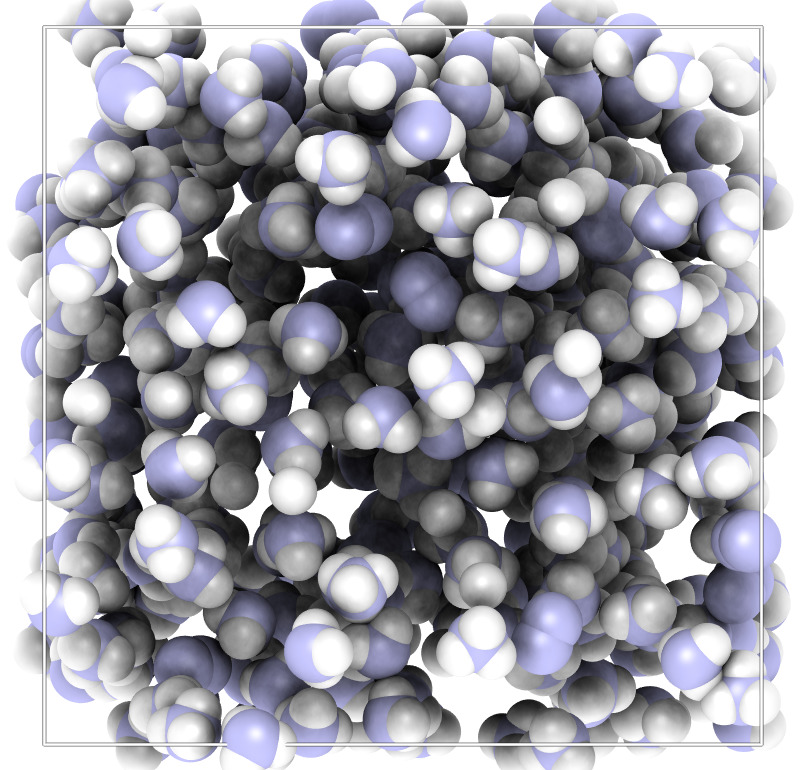
\includegraphics[width=7.5cm]{./Tutorial/Ammonia-system.jpg}}
  \subfloat[]{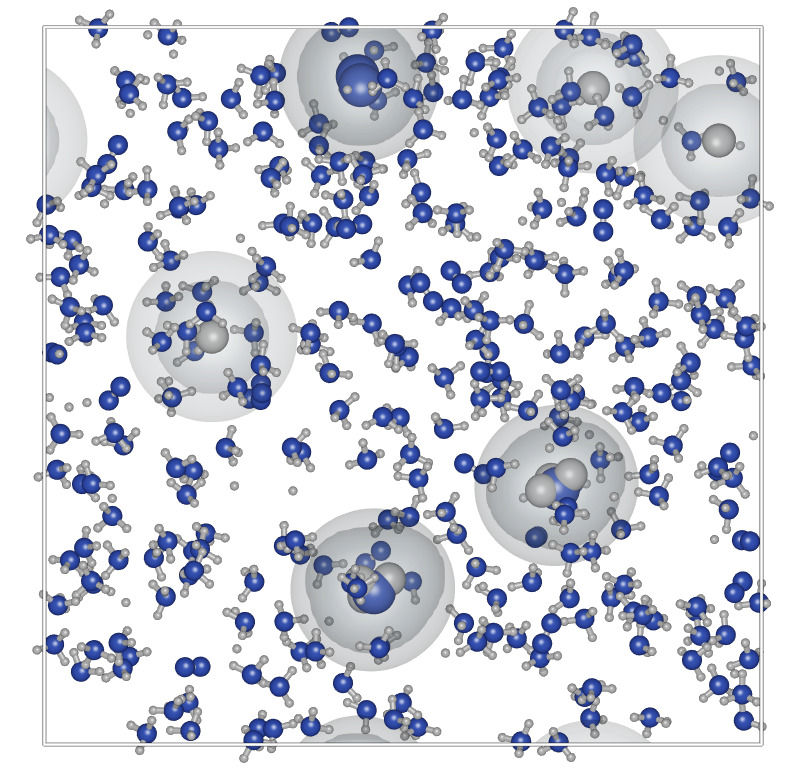
\includegraphics[width=7.5cm]{./Tutorial/Ammonia-fractional.jpg}}
  \caption{(left) the N$_2$-3H$_3$-2NH$_3$ system, (right) the fractional molecules involved in the reaction.}
  \label{Tutorial-reaction-system}
\end{figure}

Figure \ref{Tutorial-reaction-system} shows a snapshot of the N$_2$-3H$_3$-2NH$_3$ system. To efficiently
perform the reaction we use the reaction-ensemble using continuous fractional component MC. The reaction is performed
along a $\lambda$-parameter from 0 to 1, where 0 denotes the full N$_2$-3H$_3$ reactant state for the fractional components and
1 the full product state 2NH$_3$. Using fractional molecules for each component the reaction can be
performed gradually. In addition to the usual thermalization moves we have a $\lambda$-move that attempts to
change $\lambda$ with three possible outcomes:
\begin{enumerate}
\item{$\lambda$ remains between 0 and 1.}
\item{$\lambda$ goes beyond 1.}\\
We have formed real 2NH$_3$ molecules and choose new fractional molecule (randomly) with a value $\lambda-1$.
\item{$\lambda$ goes below 0.}\\
We have formed real N$_2$-3H$_3$ molecules and choose new fractional molecule (randomly) with a value $\lambda+1$.
\end{enumerate}
The $\lambda$-moves are switched on by the '\verb+ProbabilityCFCRXMCLambdaChangeMove+' input-parameter. We
also perform volume moves to impose the pressure using '\verb+VolumeChangeProbability+' option.
The example input below defines the box, the 3 components, and the reaction using
\begin{verbatim}
 Reaction 1 3 0 0 0 2 
\end{verbatim}
which list the stoichiometry of the reactants and the product. So, 1 of component 0 and 3 of component 1 forms 2
molecules of component 2.


\begin{verbatim}
SimulationType                MC
NumberOfCycles                15000
NumberOfInitializationCycles  10000
NumberOfEquilibrationCycles   20000
RestartFile                   no
PrintEvery                    500

ChargeMethod                  Ewald
Forcefield                    Local
CutOffVDW                     9.0
CutOffCoulomb                 9.0
EwaldPrecision                1e-5


Box 0
BoxLengths  38  38   38
ExternalTemperature 573.0
ExternalPressure 3e7


Reaction 1 3 0 0 0 2

ProbabilityCFCRXMCLambdaChangeMove 1.0
VolumeChangeProbability            0.1

Component 0 MoleculeName             N2
            MoleculeDefinition       Local
            LnPartitionFunction      208.188
            TranslationProbability   40.0
            RotationProbability      53.9
            ReinsertionProbability   5.0
            ExtraFrameworkMolecule   no
            CreateNumberOfMolecules  13

Component 1 MoleculeName             H2
            MoleculeDefinition       Local
            LnPartitionFunction      93.9084
            TranslationProbability   40.0
            RotationProbability      53.9
            ReinsertionProbability   5.0
            ExtraFrameworkMolecule   no
            CreateNumberOfMolecules  39

Component 2 MoleculeName             NH3
            MoleculeDefinition       Local
            LnPartitionFunction      253.69
            TranslationProbability   40.0
            RotationProbability      53.9
            ReinsertionProbability   5.0
            ExtraFrameworkMolecule   no
            CreateNumberOfMolecules  134
\end{verbatim}


\begin{figure}[H]
  \centering
\subfloat[Experiments]{
\begin{tabular}{l|l|l|l|l}
P [bar] &   573K & 673K & 773K  & 873K\\
\hline
100  &  0.53 &  0.25 &  0.10  & 0.05\\
200  &  0.67 &  0.39 &  0.18  & 0.09\\
300  &  0.75 &  0.48 &  0.25  & 0.13\\
400  &  0.80 &  0.55 &  0.32  & 0.16\\
500  &  0.84 &  0.61 &  0.37  & 0.20\\
600  &  0.87 &  0.66 &  0.42  & 0.24\\
700  &  0.89 &  0.70 &  0.47  & 0.27\\
800  &  0.91 &  0.74 &  0.51  & 0.31\\
900  &  0.93 &  0.77 &  0.55  & 0.34\\
1000 &  0.94 &  0.80 &  0.58  & 0.37\\
\hline
\end{tabular}}
\hspace{2cm}
\subfloat[Simulations]{
\begin{tabular}{l|l|l|l|l}
P [bar] &   573K & 673K & 773K  & 873K\\
\hline
100 & 0.56 & 0.27 & 0.12 & 0.05\\
200 & 0.69 & 0.41 & 0.20 & 0.09\\
300 & 0.78 & 0.49 & 0.26 & 0.14\\
400 & 0.82 & 0.57 & 0.32 & 0.17\\
500 & 0.86 & 0.62 & 0.37 & 0.20\\
600 & 0.88 & 0.66 & 0.42 & 0.24\\
700 & 0.90 & 0.69 & 0.45 & 0.27\\
800 & 0.91 & 0.73 & 0.50 & 0.30\\
900 & 0.93 & 0.77 & 0.53 & 0.33\\
1000 & 0.94 & 0.79 & 0.56 & 0.35\\
\hline
\end{tabular}}
\caption{Mol-fractions of the NH$_3$ in the ammonio bulk phase reaction of N$_2$ and H$_2$
 computed from simulation compared to experiments over a wide range of temperatures
and pressures.}
\end{figure}


\begin{table}[H]
\centering
\begin{tabular}{l|l|l|l|l}
T [K] &   N$_2$ & H$_2$ & NH$_3$ & Eq. constant K$_p$\\
\hline
573 & 2.60E+90 & 6.08E+40 & 1.50E+110 & 0.006327104\\
673 & 6.89E+77 & 1.28E+35 & 5.42E+94 & 0.000244159\\
773 & 3.44E+68 & 8.28E+30 & 2.12E+83 & 2.06653E-05\\
873 & 2.42E+61 & 5.08E+27 & 3.65E+74 & 2.97405E-06\\
\hline
\end{tabular}
\caption{Input partition function in units of \AA$^3$ and the equilibrium constant K$_p$.
The partition functions are computed based on the vibrational and rotational constants reported in the book by McQuarrie \cite{McQuarrie2000}.}
\label{Tutorial reaction-input}
\end{table}



\begin{center}
\shadowbox{%
\begin{minipage}[c]{15cm}
Exercise 1: go to the sub-directory '\verb+Tutorial/ReactionEnsembleAmmonia+'.
Using the input-parameters of Table \ref{Tutorial reaction-input} reproduce the simulation results.
\end{minipage}}
\end{center}

\bibliographystyle{Tutorial/jpc}
\bibliography{Tutorial/biblio}
